\subsubsection{Drag}
	(Insert some description of CFD methods).
	CFD was performed on the pod to determine how the pod drag coefficient varies with Mach number.
	\begin{figure}
		\centering
		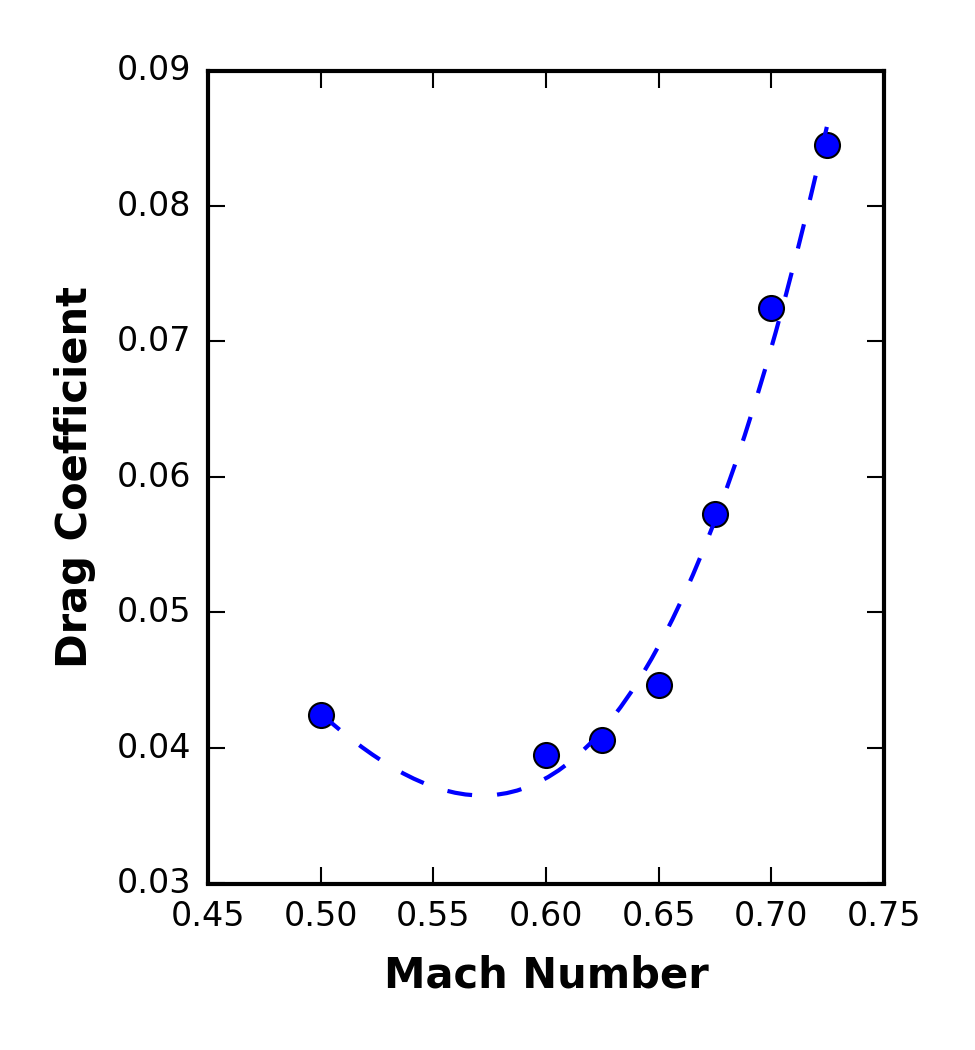
\includegraphics{../../images/graphs/cd_vs_mach/cd_vs_mach.png}
		\caption{Drag Coefficient vs. Mach Number}
		\label{fig:cd_vs_mach}
	\end{figure}
	\Cref{fig:cd_vs_mach} shows the CFD results for drag coefficient vs. Mach number.
	These results fit the trend expected for transonic flow given by the
	Prandtl-Glauert relationship. Drag Coefficient values will be interpolated
	from this data for each Mach number the system analyzes.
\subsubsection{Cycle}
	The on-board compression system provides a means of increasing the maximum
	pod speed over a closed pod,  and provides a small amount of thrust.
	A thermodynamic analysis of the compressor system is necessary to estimate
	on- board power requirements and overall heat rise of each pod.
	The compression cycle is comprised of an inlet, compressor, duct, nozzle,
	and shaft that's connected to the electric motor drivetrain. The design
	deviates from the original Hyperloop proposal by removing two heat
	exchangers as well as the air-bearings. The system is modeled as a
	one-dimensional cycle, representing components as thermodynamic processes
	that are subsequently chained together. Each component is responsible for
	calculating gas properties across its boundaries and appropriately enforcing
	conservation equations across the entire system.
\subsubsection{Drivetrain}
	The Drivetrain module models an electric motor, inverter, and battery system.
	Building off of previous work done at Georgia Tech and NASA, the module
	will compute the size and mass of both the motor and battery system
	neccesery to sustain the mission based on required torque and power demands
	over a mission profile \cite{GeorgiaTechMotor, NASASugar}. The model
	utilizes a modified algorithm for sizing the battery from the algorithm
	developed at NASA by MK Bradley et. al. With the modification that the
	voltage of the battery as a function discharge is modeled using a
	polynomial fit to discharge curves provided by cell manufacturers \cite{NASASugar}.
	This change provides results that are more flexible and specific to the
	leading commercial battery cells.
\subsubsection{Geometry and Mass}
	In order to analyze the design of the tube structure, the final mass and
	geometric configuration of the pod must be obtained. The geometry model
	assumes the pod to have a cylindrical fuselage with conical frustrums at
	the inlet and exit. The cross sectional area of the passenger section
	given by the user is added to the cross sectional area of the compressor
	exit duct, which is computed in the cycle analysis. The geometry module
	also estimates the thickness of the pod wall and the passenger compartment
	based on simple pressurized cylinder relationships, then adds these areas
	together to compute the total cross sectional area. The length of each
	component is also fed into the geometry model so it can compute the total
	pod length and planform area. The mass module takes the mass of each
	component and adds them with the total passenger mass in order to determine
	the mass of the pod without magnets for levitation. The Levitation component
	takes in this mass, computes the mass of the magnets, then outputs the total mass of the pods.
\subsubsection{Pod Mach}
	\begin{table}[ht]
	\caption{Tube Power Variables} % title of Table
	\centering % used for centering table
	\begin{tabular}{c c c} % centered columns (4 columns)
	\hline\hline %inserts double horizontal lines
	Symbol & Variable & Units \\ [0.5ex] % inserts table
	%heading
	\hline % inserts single horizontal line
	$A$ & Area& m^{2}\\
	$A^{*}$ & Throat Area& m^{2}& none\\
	$M$ & Mach number& none\\
	$\gamma$ & Ratio of specific heats& none\\
	$P_{crit}$ & Critical pressure at which bucking occurs & Pa\\
	$E$ &Elastic modulus& Pa\\
	$\nu$ & Poisson Ratio& none\\
	$t$ & Thickness & m\\
	$r$ & Radius & m\\
	$\delta^{*}$ & Displacement boundary layer thickness & m\\
	$x$ & Distance in x direction & m\\
	$Re_{x}$ & Length based Reynolds number & none\\
	$\varepsilon$ & expansion ratio & none\\
	$L$ & Track Length & m\\\
	$ib$ & Bond interest rate & none\\
	$bm$ & Bond maturity & years\\
	$g$ & Gravitational acceleration & m/s^{2}\\
	$v$ & velocity & m/s
	$F_{x}$ & Magnetic Drag & N\\
	$m$ & Mass & kg\\
	$\alpha$ & weighing factor\\
	\hline %inserts single line
	\end{tabular}
	\label{table:nonlin} % is used to refer this table in the text
	\end{table}
	The pod mach module uses the pod cross-sectional area, Mach number, and
	compressor inlet conditions to compute the tube area. As the pod travels,
	flow that is not entrained by the compressor must accelerate around the pod.
	Due to the pod’s transonic flight speed, it is possible that this bypass
	flow could accelerate to Mach 1 and cause the flow to choke, which would
	lead to an undesirable buildup of pressure in front of the pod and
	increased drag. To avoid this condition, this module sizes the tube area
	such that there is a large enough bypass area to prevent the bypass flow
	from accelerating to Mach 1. This is done using a simple quasi 1D area
	relationship for compressible flow given by the equation
	\begin{equation}
		\label{eq:mach_to_area}
		\frac{A_{1}}{A_{2}}=\frac{M_{2}}{M_{1}} \left( \frac{1+\frac{\gamma -1}{2}M_{1}^{2}}{1+\frac{\gamma -1}{2}M_{2}^{2}} \right)^{\frac{( \gamma +1 )}{2 ( \gamma -1  )}}
	\end{equation}
	For this analysis, $M_1$ is the free stream Mach number, $M_2$ is the
	desired bypass Mach number, $A_1$ is the initial area of the bypass flow
	($A_{tube}$ - $A_{inlet}$), and $A_2$ is the bypass area ($A_{tube}$ - $A_{pod}$).
	For these analyses, $M_2$ is set to .95 in order to provide a slight factor
	of safety to prevent the flow from reaching the choking condition.
	In order to make this model higher fidelity, it is possible to modify the
	areas in the relationship to account for boundary layer development over
	the pod outer surface. As the boundary develops, the effective bypass area
	is reduced which increases the risk of bypass flow reaching Mach 1. However,
	it is possible to modify this by increasing the effective pod radius by the
	displacement thickness of the boundary layer. The sensitivity of structural
	design to boundary layer growth is important and will be discussed at length later.
\subsubsection{Levitation}
	\begin{table}[ht]
	\caption{Symbols Used in Levitation Equations}
	\centering
	\begin{tabular}{c c c}
	\hline\hline
	Symbol & Use & Units\\ [0.5ex]
	\hline
	$\lambda$ & Wavelength of Halbach Array & m\\
	$w$ & Width of the Magnetic Array & m\\
	$\beta _{0}$ & Halbach Peak Strength & Tesla\\
	$R$ & Resistance of the Track & $\Omega$\\
	$L$ & Inductance of the Track & Henry\\
	$\omega$ & Frequency of the Induced Current & Hz\\
	$h$ & Desired Levitation Height & m\\
	$g$ & Gravity & $m/s^{2}$\\
	$A$ & Area of Magnetic Array & $m^{2}$\\
	$v$ & Velocity of the Pod & $m/s$\\ [1ex]
	\hline
	\end{tabular}
	\label{table:nonlin}
	\end{table}
	The Hyperloop concept operates using a levitation system to significantly
	reduce friction during high velocity areas of travel. In this analysis, a
	passive magnetic levitation system is used to suspend the pod above the
	track as it travels. The passive system is advantageous because it requires
	zero power input for levitation to occur, which is advantageous when
	traveling over long distances. The Inductrack passive levitation method
	developed at the Lawrence Livermore National Laboratory is chosen as the
	system for our Hyperloop model \cite{inductrack}. Some assumptions were
	taken to simplify the analysis adapted from this model. It is assumed that
	ferrite tiles were not used so that the added inductive loading is set to
	zero, leaving only the distributed inductance to computed in the model.
	Fringe fields from the magnetic array are also ignored in this analysis and
	the width of the magnetic array is set equal to the width of the track.
	These three simplifications and assumptions allow the overall scale factor
	for the total force, $levsf$, to set equal to unity.

	The levitation group makes two critical calculations: the inductance of the
	track required for the pod to levitate at a desired speed and the mass of
	the permanent magnets onboard. The breakpoint levitation module uses a
	desired minimum levitation speed and uses it to calculate important track
	parameters, including the ratio of inductance to resistance of the track.

	Using a desired levitation speed, the total mass of magnets required and
	drag force produced is is then calculated. The lift and drag produced
	produced by the magnets are given in the equations
	\begin{equation}
		\label{eq:fy_lev}
		F_{y}(\omega)=[\beta _{0}^{2}w/(4\pi Ldc\lambda )][( 1+R/\omega L)(1+R/\omega L)^{2})]Ae^{-4\pi h/\lambda }
	\end{equation}
	\begin{equation}
		\label{eq:dmag}
		D_{mag}=( m_{pod}g)R/\omega L
	\end{equation}
	In these equations, the drag and the magnet mass are both functions of the
	magnet area and thickness. To minimize drag and mass, a Pareto optimization
	is performed prior to running the system model. The following cost function
	is developed by normalizing drag and mass, then multiplying by a weighing
	factor $alpha$ and adding them together in the following equation
	\begin{equation}
		\label{eq:pareto}
		f(\alpha ) = \alpha \bar{F_{x}} + (1-\alpha )\bar{m_{mag}}v
	\end{equation}
	Where the bar signifies the normalized value. The weighing factor $alpha$
	is chosen arbitrarily between zero and unity; high values of $alpha$
	emphasize minimizing drag while low values of $alpha$ emphasize minimizing mass.




